
\documentclass[
	% -- opções da classe memoir --
	article,			% indica que é um artigo acadêmico
	11pt,				% tamanho da fonte
	oneside,			% para impressão apenas no verso. Oposto a twoside
	a4paper,			% tamanho do papel. 
	% -- opções da classe abntex2 --
	%chapter=TITLE,		% títulos de capítulos convertidos em letras maiúsculas
	%section=TITLE,		% títulos de seções convertidos em letras maiúsculas
	%subsection=TITLE,	% títulos de subseções convertidos em letras maiúsculas
	%subsubsection=TITLE % títulos de subsubseções convertidos em letras maiúsculas
	% -- opções do pacote babel --
	english,			% idioma adicional para hifenização
	brazil,				% o último idioma é o principal do documento
	sumario=tradicional
	]{abntex2}


\usepackage{lmodern}			% Usa a fonte Latin Modern
\usepackage[T1]{fontenc}		% Selecao de codigos de fonte.
\usepackage[utf8]{inputenc}		% Codificacao do documento (conversão automática dos acentos)
\usepackage{indentfirst}		% Indenta o primeiro parágrafo de cada seção.
\usepackage{nomencl} 			% Lista de simbolos
\usepackage{color}				% Controle das cores
\usepackage{graphicx}			% Inclusão de gráficos
\usepackage{microtype} 			% para melhorias de justificação
\usepackage{multicol}
\setlength{\columnsep}{0,5cm}


\usepackage[brazilian,hyperpageref]{backref}	 % Paginas com as citações na bibl
\usepackage[alf]{abntex2cite}	% Citações padrão ABNT
% ---
\renewcommand{\backrefpagesname}{Citado na(s) página(s):~}
% Texto padrão antes do número das páginas
\renewcommand{\backref}{}
% Define os textos da citação
\renewcommand*{\backrefalt}[4]{
	\ifcase #1 %
		Nenhuma citação no texto.%
	\or
		Citado na página #2.%
	\else
		Citado #1 vezes nas páginas #2.%
	\fi}%


\definecolor{blue}{RGB}{41,5,195}

% informações do PDF
\makeatletter
\hypersetup{
     	%pagebackref=true,
		pdftitle={\@title}, 
		pdfauthor={\@author},
    	pdfsubject={Modelo de artigo científico com abnTeX2},
	    pdfcreator={LaTeX with abnTeX2},
		pdfkeywords={abnt}{latex}{abntex}{abntex2}{atigo científico}, 
		colorlinks=true,       		% false: boxed links; true: colored links
    	linkcolor=blue,          	% color of internal links
    	citecolor=blue,        		% color of links to bibliography
    	filecolor=magenta,      		% color of file links
		urlcolor=blue,
		bookmarksdepth=4
}

\setlrmarginsandblock{3cm}{3cm}{*}
\setulmarginsandblock{3cm}{3cm}{*}
\checkandfixthelayout
\setlength{\parindent}{1.3cm}
\setlength{\parskip}{0.2cm}  % tente também \onelineskip

% Espaçamento simples
\SingleSpacing
\usepackage{graphicx}
\usepackage{subcaption}
%codigo
\usepackage{listings}
\usepackage{xcolor}


\begin{document}
\frenchspacing 

\titulo{Experimento com Métodos de Ordenação}
\autor{Giovana Piazza \and Rodrigo Peraça}
\local{Universidade Federal do Pampa - Bagé - Rio Grande do Sul}


\maketitle

\begin{abstract}
Este trabalho realiza uma análise comparativa de diversos algoritmos de ordenação, incluindo métodos clássicos (Bubble, Insertion, Selection, Shell, Heap, Merge e Quick Sort) e lineares (Counting, Radix e Bucket Sort) \cite{devmedia_algoritmos_ordenacao_java}. O desempenho foi avaliado em diferentes tamanhos e tipos de vetores (crescente, decrescente e aleatório), relacionando os resultados à complexidade assintótica de cada algoritmo. Os experimentos mostraram diferenças significativas de tempo de execução, evidenciando a importância da escolha adequada do algoritmo conforme o volume e a organização dos dados.
\end{abstract}

\section{Introdução}
Os algoritmos de ordenação são fundamentais na ciência da computação, sendo amplamente utilizados em aplicações que envolvem organização de dados e otimização de consultas. Diferentes métodos apresentam características próprias quanto à eficiência, complexidade e comportamento em relação ao tipo de entrada fornecida.

Neste trabalho, são analisados diversos algoritmos clássicos de ordenação, incluindo os métodos quadráticos (\textit{Bubble Sort}, \textit{Insertion Sort}, \textit{Selection Sort}), métodos baseados em divisão e conquista (\textit{Merge Sort}, \textit{Quick Sort}, \textit{Heap Sort} e \textit{Shell Sort}), e métodos lineares ou quase lineares (\textit{Counting Sort}, \textit{Radix Sort} e \textit{Bucket Sort}). O objetivo é avaliar empiricamente o tempo de execução de cada um, considerando diferentes cenários de entrada e tamanhos de vetor.
\cite{unipampa_algoritmos_classificacao_dados}

\section{Metodologia}
Cada algoritmo foi executado 20 vezes para reduzir variações ocasionais de desempenho do sistema, e as médias dos tempos foram calculadas em nanossegundos, sendo posteriormente convertidas para milissegundos.

Foram utilizados vetores de diferentes tamanhos (100, 1.000, 10.000, 100.000 e 1.000.000 elementos e em três configurações distintas: crescente, decrescente e aleatória). Essa diversidade de casos possibilita uma análise mais abrangente sobre a escalabilidade e o comportamento de cada método em situações práticas.

\section{Código}
\subsection{Geral}
Para avaliar o desempenho dos métodos de ordenação, foi desenvolvido um programa em Java que integra todas as implementações e permite ao usuário selecionar qual algoritmo aplicar a um conjunto de dados. O arquivo Main.java funciona como ponto de entrada, garantindo execução padronizada e interação controlada com o sistema.

O código é modular, com cada algoritmo encapsulado em métodos da classe Ordenadores, facilitando a comparação entre eles em termos de complexidade e comportamento prático. Além disso, o programa possibilita medir empiricamente o tempo de execução para diferentes tamanhos e tipos de vetores, servindo como ferramenta de experimentação e análise das diferenças de desempenho entre os algoritmos.

\subsection{Bublle Sort}
O algoritmo Bubble Sort é um dos métodos de ordenação mais simples e didáticos. Seu funcionamento baseia-se na comparação sucessiva de pares adjacentes de elementos, trocando-os de posição sempre que estiverem fora de ordem. A cada passagem completa pelo vetor, o maior elemento “flutua” para a última posição, como uma bolha que sobe à superfície — daí o nome do algoritmo.
Apesar de ser de fácil implementação, o Bubble Sort apresenta desempenho insatisfatório para grandes conjuntos de dados, com complexidade de tempo quadrática O($n^2$) no pior caso. Entretanto, quando o vetor já está parcialmente ordenado, é possível otimizar o processo interrompendo a execução caso nenhuma troca ocorra em uma passagem, o que reduz o tempo para O(n) no melhor caso. Trata-se de um algoritmo estável, mas pouco eficiente para aplicações práticas.
    
\subsection{Insertion Sort}
O Insertion Sort é um algoritmo de ordenação simples e eficiente para conjuntos de dados pequenos ou parcialmente ordenados. Sua lógica simula o modo como uma pessoa organiza cartas na mão: cada novo elemento é inserido na posição correta em relação aos anteriores.
O método percorre o vetor da esquerda para a direita, comparando o elemento atual com os anteriores e deslocando-os até encontrar o local apropriado para inserção.
Seu desempenho médio e pior é de O($n^2$), enquanto o melhor caso (vetor já ordenado) atinge O(n). É um algoritmo estável e in-place, ou seja, não requer memória adicional além do vetor original. Por essas características, é frequentemente utilizado como sub-rotina em algoritmos mais complexos, como o Quick Sort e o Shell Sort, quando as partições tornam-se pequenas.

\subsection{Selection Sort}
O Selection Sort baseia-se na ideia de selecionar repetidamente o menor elemento do subconjunto não ordenado e colocá-lo na posição correta. A cada iteração, o algoritmo encontra o mínimo restante e o troca com o elemento da posição atual.
Dessa forma, após a primeira passagem, o menor elemento ocupa a primeira posição; após a segunda, o segundo menor, e assim por diante.
Apesar de realizar apenas n−1 trocas (o que pode ser vantajoso quando o custo de escrita é alto), o número de comparações permanece fixo em O($n^2$). O Selection Sort não é estável, pois trocas diretas podem alterar a ordem relativa de elementos iguais. É simples de entender, mas pouco eficiente para grandes volumes de dados.

    
\subsection{Shell Sort}
O Shell Sort é uma melhoria do Insertion Sort, desenvolvida por Donald Shell. Ele introduz a ideia de “intervalos” (ou gaps), permitindo que elementos distantes sejam comparados e movidos antes da ordenação final.
Inicialmente, o vetor é dividido em várias sublistas formadas por elementos espaçados por um determinado gap. Cada sublista é ordenada usando o Insertion Sort. O gap é então reduzido progressivamente até que se torne igual a 1, momento em que o vetor já estará quase ordenado, e uma última ordenação garante o resultado final.
Com uma escolha adequada da sequência de gaps, o desempenho pode se aproximar de O($n^{3/2}$) ou melhor, tornando-o significativamente mais rápido que os algoritmos quadráticos tradicionais. O Shell Sort não é estável, mas é um algoritmo in-place e prático para conjuntos médios de dados.

\subsection{Heap Sort}
O Heap Sort utiliza a estrutura de dados heap (uma árvore binária completa que satisfaz a propriedade de heap) para ordenar elementos. Primeiramente, o vetor é reorganizado de forma a representar um max-heap, onde o maior elemento está na raiz.
Em seguida, o maior elemento é removido (trocado com o último elemento do vetor) e o tamanho do heap é reduzido. O processo é repetido até que todos os elementos estejam ordenados.
O Heap Sort apresenta desempenho garantido de O(nlogn) tanto no melhor quanto no pior caso, sendo uma boa opção quando é necessário um tempo de execução previsível. Contudo, ele não é estável e tende a ser mais lento que o Quick Sort na prática devido a acessos menos eficientes à memória. É um algoritmo in-place, pois utiliza apenas o vetor original.

\subsection{Merge Sort}
O Merge Sort é um algoritmo baseado na técnica de divisão e conquista. O vetor é recursivamente dividido em duas metades até restarem subvetores de um único elemento. Em seguida, essas metades são intercaladas (merge) em ordem crescente, produzindo vetores cada vez maiores e ordenados.
Esse processo garante um desempenho consistente de O(nlogn) em todos os casos, tornando o Merge Sort especialmente adequado para grandes volumes de dados.
Sua principal desvantagem é o uso adicional de memória, já que a intercalação requer um vetor auxiliar. Por outro lado, é um algoritmo estável e de comportamento previsível, o que o torna uma escolha comum em bibliotecas padrão e aplicações que exigem estabilidade na ordenação.

\subsection{Quick Sort}
O Quick Sort é um dos algoritmos de ordenação mais eficientes em prática. Também baseado em divisão e conquista, ele seleciona um elemento pivô e particiona o vetor em duas partes: uma contendo elementos menores que o pivô e outra com os maiores.
O processo é aplicado recursivamente a cada partição até que o vetor esteja ordenado.
A escolha do pivô é determinante para o desempenho do algoritmo: uma escolha ruim pode levar ao pior caso de O($n^2$), mas técnicas como a mediana de três ou pivôs aleatórios geralmente garantem O(nlogn) em média.
O Quick Sort é in-place, mas não é estável. Devido à sua eficiência prática e boa localidade de memória, é amplamente utilizado em sistemas reais, sendo a base de várias implementações modernas, como o Dual-Pivot Quick Sort do Java.

\subsection{Bucket Sort}
O Bucket Sort (ou ordenação por baldes) distribui os elementos em um conjunto de “baldes” (ou intervalos) com base em suas chaves. Cada balde é então ordenado individualmente — geralmente usando Insertion Sort — e, por fim, todos são concatenados para formar o vetor final.
Quando os dados estão uniformemente distribuídos, o algoritmo pode atingir desempenho quase linear O(n+k). No entanto, em casos desfavoráveis (quando muitos elementos se concentram em poucos baldes), o tempo pode crescer até O($n^2$).
O Bucket Sort é adequado para dados reais distribuídos em intervalos conhecidos, como números de ponto flutuante em [0, 1). É um método intuitivo e eficiente, especialmente em combinações híbridas com outros algoritmos.


\subsection{Counting Sort}
O Counting Sort é um algoritmo de ordenação não comparativo, ideal para conjuntos de dados numéricos em intervalos limitados. Ele opera contando o número de ocorrências de cada valor e, em seguida, utilizando essas contagens para determinar as posições finais dos elementos.
Como não realiza comparações diretas, o Counting Sort pode alcançar complexidade linear O(n+k), onde k é o valor máximo das chaves.
É estável quando implementado corretamente e muito eficiente para intervalos pequenos de valores. Entretanto, torna-se inviável quando as chaves possíveis são muito dispersas, devido à necessidade de um vetor auxiliar proporcional ao tamanho do intervalo.

\subsection{Radix Sort}
O Radix Sort também é um algoritmo não comparativo, que ordena os elementos processando-os dígito a dígito. Ele normalmente utiliza o Counting Sort como sub-rotina estável para ordenar os números de acordo com cada dígito, do menos significativo (LSD) ao mais significativo (MSD).
A complexidade do Radix Sort é O(d⋅(n+k)), onde d representa o número de dígitos e k o tamanho da base numérica usada.
Esse método é extremamente eficiente quando o número de dígitos é pequeno em relação ao tamanho do conjunto. Contudo, exige espaço adicional e é restrito a dados que possam ser decompostos em chaves posicionais, como inteiros ou strings.
Quando combinado com um Counting Sort estável, o Radix Sort mantém a estabilidade e apresenta desempenho linear.

\section{Comparação Vetores}
Todos os algoritmos foram executados 20 vezes para cada tamanho de vetor, garantindo médias confiáveis. Os testes consideraram vetores de 100 a 1.000.000 elementos, em ordem crescente, decrescente e aleatória, permitindo avaliar a escalabilidade e comparar o desempenho entre algoritmos de diferentes complexidades.

\subsection{Vetor aleatório}
É possível notar diferenças significativas entre os métodos quadráticos (Bubble Sort, Insertion Sort, Selection Sort), métodos de melhoria intermediária (Shell Sort), métodos baseados em divisão e conquista (Merge Sort, Quick Sort, Heap Sort) e algoritmos lineares ou quase lineares (Counting Sort, Radix Sort, Bucket Sort).

Os algoritmos quadráticos apresentam tempos de execução muito maiores e maior variabilidade, especialmente em vetores de grande porte, devido ao elevado número de comparações e trocas necessárias. Já os métodos de divisão e conquista mantêm desempenho mais consistente, pois partem o problema em subproblemas menores, diminuindo o número de operações. Os algoritmos lineares ou quase lineares se destacam por apresentar tempos baixos e estáveis, uma vez que sua complexidade depende diretamente do tamanho do vetor ou do intervalo de valores, permitindo processar grandes quantidades de dados de forma eficiente.

\begin{figure}[h!]
    \centering
    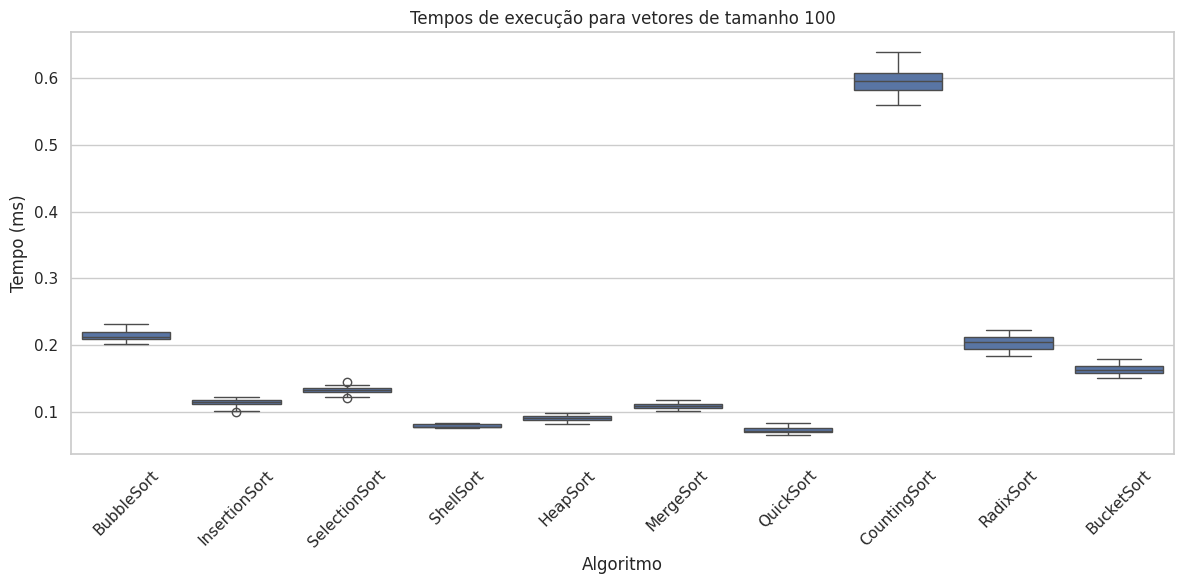
\includegraphics[width=1\linewidth]{Tempo100.png}
    \caption{Vetor com 100 entradas}
    \label{fig:placeholder}
\end{figure}

\begin{figure}[h!]
    \centering
    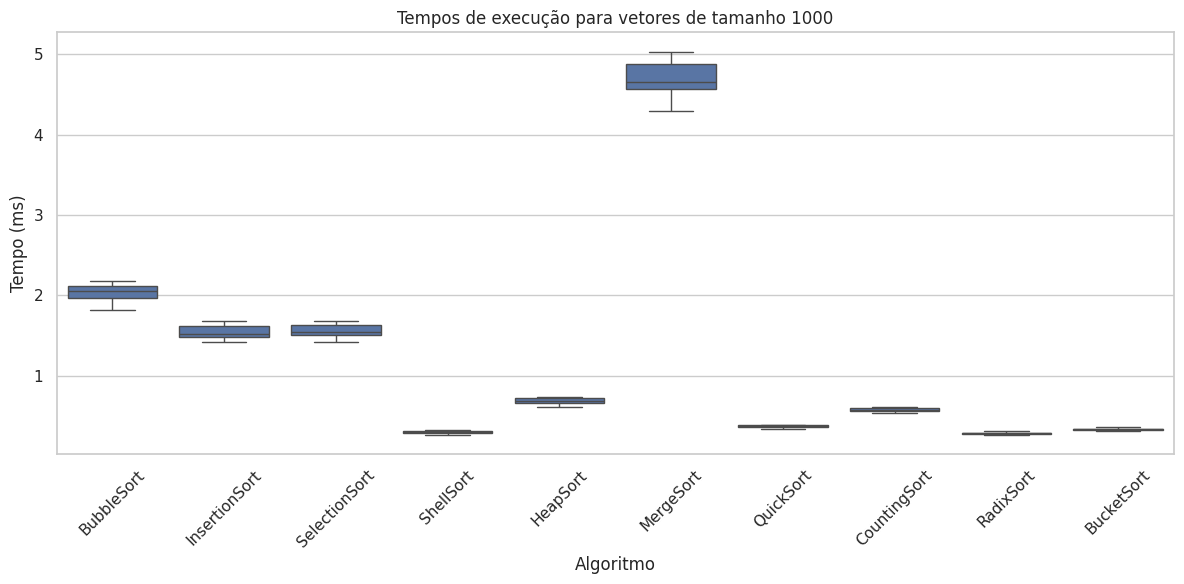
\includegraphics[width=1\linewidth]{Tempo1000.png}
    \caption{Vetor com 1000 entradas}
    \label{fig:placeholder}
\end{figure}


\begin{figure}[h!]
    \centering
    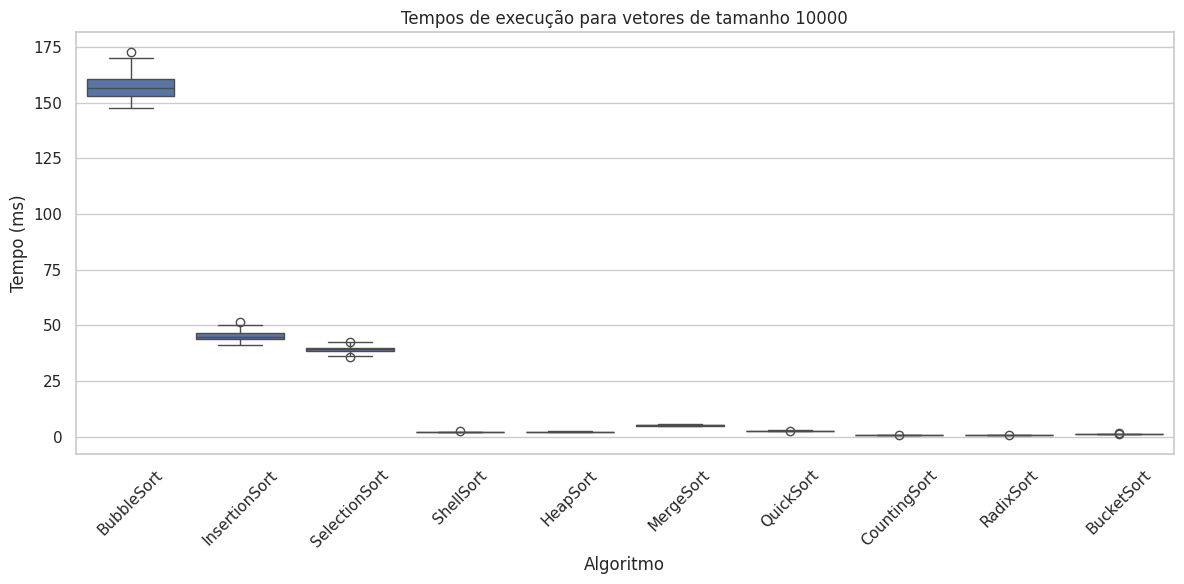
\includegraphics[width=0.9\linewidth]{Tempo10000.png}
    \caption{Vetor com 10000 entradas}
    \label{fig:placeholder}
\end{figure}

\begin{figure}[h!]
    \centering
    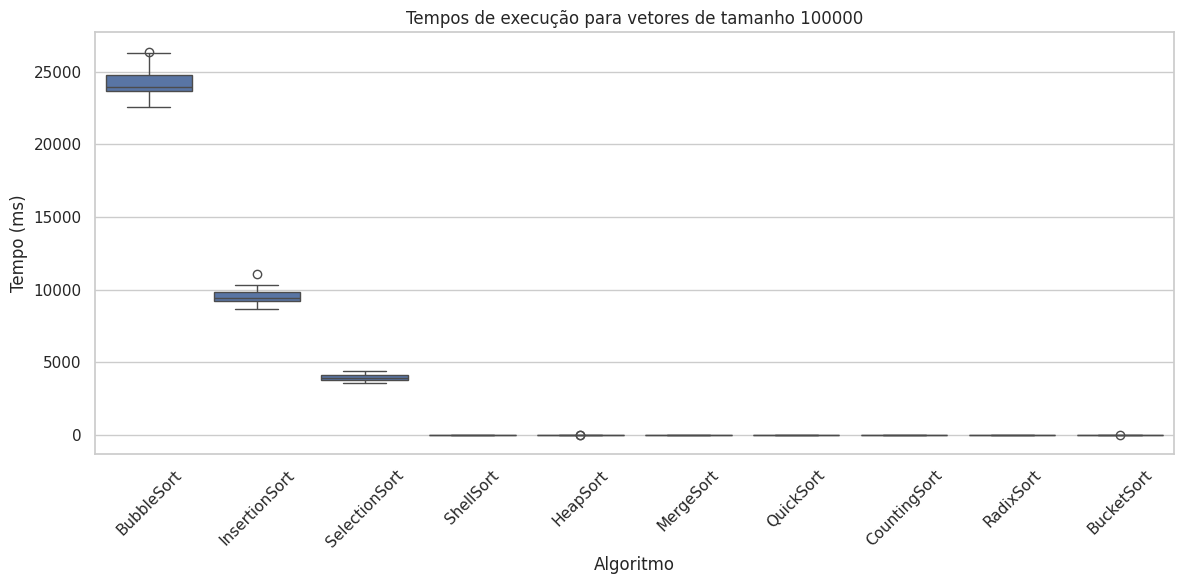
\includegraphics[width=0.9\linewidth]{Tempo100000.png}
    \caption{Vetor com 100000 entradas}
    \label{fig:placeholder}
\end{figure}

\begin{figure}[h!]
    \centering
    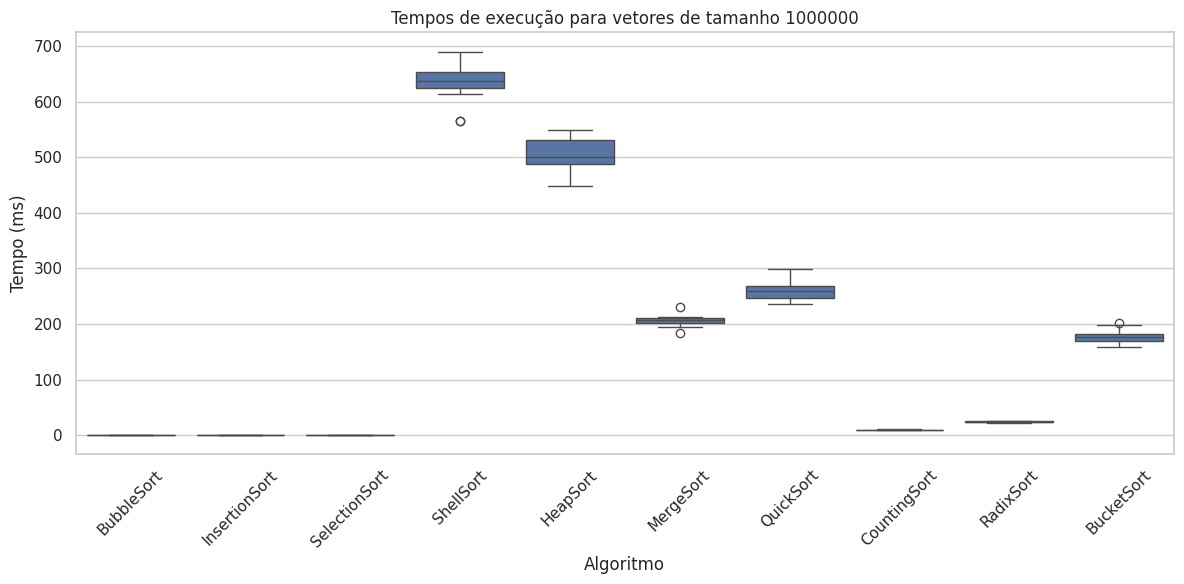
\includegraphics[width=0.8\linewidth]{Tempo1000000.png}
    \caption{Vetor com 1000000 entradas}
    \label{fig:placeholder}
\end{figure}

\subsection{Vetor Crescente}
Quando o vetor está em ordem crescente, o tempo de execução dos algoritmos de ordenação tende a ser menor, especialmente para métodos como o \textit{Insertion Sort} e o \textit{Bubble Sort}. Isso ocorre porque, nesse caso, os elementos já estão próximos de suas posições corretas, exigindo poucas ou nenhuma troca. No caso do \textit{Insertion Sort}, por exemplo, o algoritmo apenas compara os elementos sem precisar deslocá-los, resultando em um número reduzido de operações e atingindo seu melhor caso, com complexidade próxima a $O(n)$. Assim, vetores ordenados de forma crescente demandam menos esforço computacional, refletindo em tempos de execução significativamente menores.


\begin{figure}[h!]
    \centering
    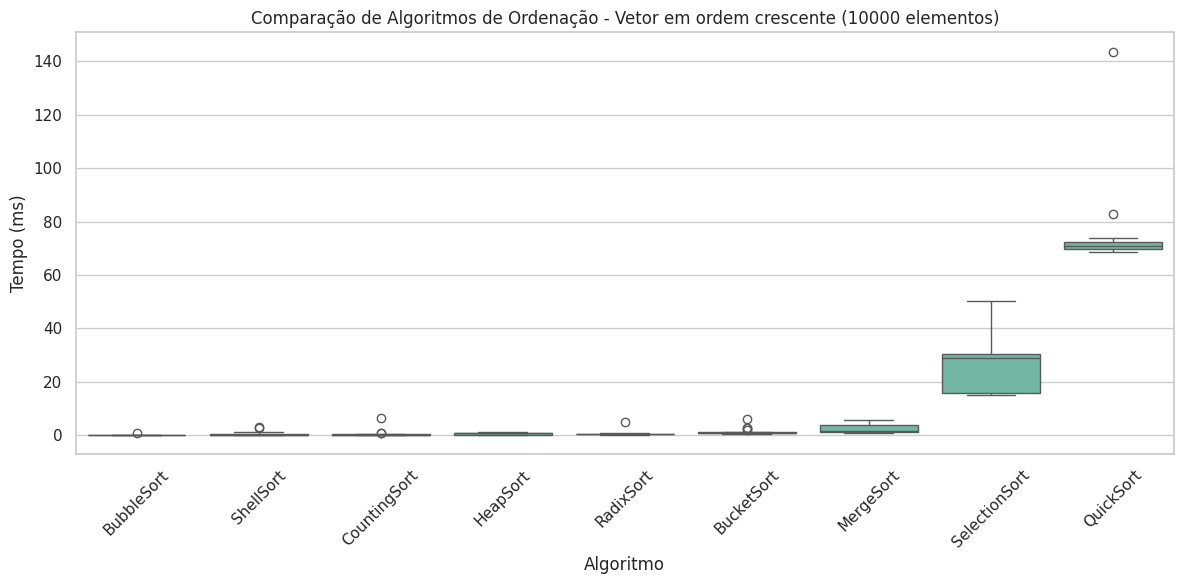
\includegraphics[width=1\linewidth]{Crescente.png}
    \caption{Tempo para um vetor de 10 mil entradas crescentes}
    \label{fig:placeholder}
\end{figure}

\subsection{Vetor Decrescente}

Quando o vetor está em ordem decrescente, o tempo de execução tende a ser maior, pois os algoritmos de ordenação precisam realizar o número máximo de comparações e trocas para reorganizar completamente os elementos. Nos métodos quadráticos, como o \textit{Bubble Sort} e o \textit{Insertion Sort}, esse cenário representa o pior caso possível, em que cada elemento precisa ser movido diversas posições até alcançar sua localização correta. Mesmo algoritmos mais eficientes, como o \textit{Quick Sort}, podem ter desempenho degradado se a escolha do pivô não for adequada, resultando em partições desbalanceadas. Dessa forma, o vetor decrescente impõe maior carga computacional e, consequentemente, tempos de execução mais elevados.

\begin{figure}[h!]
    \centering
    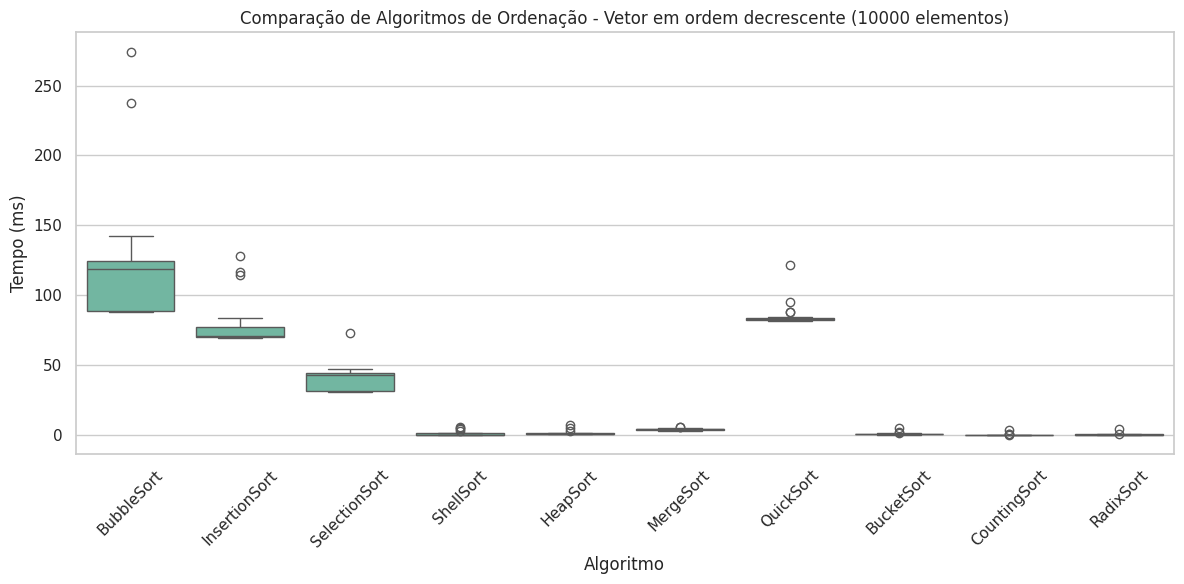
\includegraphics[width=1\linewidth]{Decrescente.png}
    \caption{Tempo para um vetor de 10 mil entradas decrescentes}
    \label{fig:placeholder}
\end{figure}

\newpage
\section{Conclusão}
A análise dos resultados obtidos evidencia diferenças expressivas entre os grupos de algoritmos quanto ao tempo de execução e à consistência dos dados. Por meio dos boxplots, foi possível visualizar a variação dos tempos, a presença de outliers e o nível de estabilidade de cada abordagem, permitindo uma comparação abrangente entre os diferentes métodos de ordenação.

Os algoritmos quadráticos, como o \textit{Bubble Sort}, \textit{Insertion Sort} e \textit{Selection Sort}, apresentaram, como esperado, os maiores tempos de execução, especialmente em vetores de grande porte. Ainda assim, o \textit{Insertion Sort} demonstrou desempenho superior nos vetores parcialmente ordenados, uma vez que o número de comparações e trocas se reduz consideravelmente em cenários crescentes. Apesar disso, tais algoritmos mantêm um comportamento previsível, mas pouco eficiente, tornando-se inadequados para grandes volumes de dados.

Os métodos baseados em divisão e conquista — \textit{Merge Sort}, \textit{Quick Sort}, \textit{Heap Sort} e \textit{Shell Sort} — apresentaram desempenho intermediário a excelente, com destaque para o \textit{Quick Sort}, que obteve os menores tempos médios em vetores aleatórios devido à boa escolha de pivôs. O \textit{Merge Sort} mostrou-se estável e previsível, enquanto o \textit{Heap Sort} manteve desempenho consistente, embora inferior ao \textit{Quick Sort} em casos médios. O \textit{Shell Sort}, por sua vez, apresentou desempenho competitivo e satisfatório, destacando-se como uma alternativa eficiente e de implementação simples. A dispersão dos tempos nesse grupo foi moderada, demonstrando boa escalabilidade e robustez.

Os algoritmos lineares e quase lineares, como o \textit{Counting Sort}, \textit{Radix Sort} e \textit{Bucket Sort}, possuem complexidade teórica inferior, o que deveria garantir tempos de execução reduzidos. No entanto, observou-se que o desempenho real desses métodos depende fortemente da implementação, do tamanho do vetor e da distribuição dos dados. Embora tenham apresentado bons tempos em muitos casos, nem sempre superaram os algoritmos de divisão e conquista, especialmente em vetores menores ou com distribuição não uniforme. Isso evidencia que a eficiência teórica nem sempre se traduz diretamente em desempenho prático, sendo necessário considerar aspectos como o custo de memória e o overhead de processamento.

De modo geral, a comparação entre os grupos permite concluir que os algoritmos quadráticos são adequados apenas para pequenos conjuntos de dados ou vetores já ordenados; os algoritmos baseados em divisão e conquista oferecem o melhor equilíbrio entre velocidade e estabilidade; e os métodos lineares, embora potencialmente mais rápidos, exigem condições ideais para alcançar o desempenho esperado.

Assim, o \textit{Quick Sort} destacou-se como o algoritmo de melhor desempenho médio, enquanto o \textit{Bubble Sort} apresentou os piores resultados, corroborando as análises clássicas da literatura. Em síntese, o comportamento prático dos algoritmos de ordenação nem sempre reflete suas complexidades teóricas, e a escolha do método mais adequado deve considerar o volume de dados, a natureza da entrada e a necessidade de previsibilidade. Essa análise empírica reforça a importância da experimentação prática na seleção do algoritmo ideal para cada contexto computacional.

\bibliography{Modelo}
\end{document}
